\section{Influenza del gruppo}
In presenza di un pericolo abbiamo tutti una naturale propensione a scappare. Questo atteggiamento, però, può subire delle variazioni se ad interessarci non è solo la nostra incolumità, ma anche quella di coloro tra i presenti con i quali abbiamo una particolare relazione affettiva. \newline
\enquote{Una famiglia sopravvive insieme o muore insieme} \cite{Kster2011} è un'affermazione che in maniera molto esplicita, sottolinea la validità di questo principio e nella quale probabilmente, tutti ci sentiamo immedesimati.

\subsection{Descrizione della simulazione}
In un ambiente euclideo continuo ed illimitato è stata inserita una fonte di pericolo al centro ed intorno ad essa sono stati disposti in maniera casuale 24 persone. \newline
Si sono effettuate due simulazioni: nella prima non considerando l'esistenza di eventuali gruppi costituiti da più agenti, mentre nella seconda specificando quattro diversi insiemi di amici di dimensioni variabili. In quest'ultimo caso, ogni agente è stato assegnato ad un gruppo senza tenere in considerazione la posizione reciproca, quindi ammettendo anche il caso di membri molto lontani tra loro nell'ambiente. \newline
Per indurre il movimento, si è scelta la reazione \texttt{BlendedSteering}, con la quale vengono uniti il meccanismo di coesione ed il comportamento di steering dell'inseguimento del flusso, rappresentante un allontanamento dalla fonte di pericolo.

\subsection{Risultati ottenuti}
Confrontando i fotogrammi della simulazione con solo pedoni solitari (figura \ref{fig:influence-without-groups}) rispetto a quelli della simulazione con gruppi di dimensioni maggiori (figura \ref{fig:influence-with-groups}), il comportamento che si riscontra è indubbiamente differente. \newline
Come era prevedibile, quando un pedone non è vincolato dalla presenza di altri membri nel suo gruppo, cerca solamente di allontanarsi il più possibile dal pericolo. \newline 
Al contrario, se è condizionato dalla necessità di ricongiungersi con qualcun altro, lo si vede muovere intorno alla zona di rischio alla sua ricerca. Solo una volta che tutto il gruppo si è ricongiunto, i vari membri che lo compongono procedono ad allontanarsi il più possibile.

\begin{figure}
    \centering
    \begin{subfigure}[b]{0.75\textwidth}
        \centering
        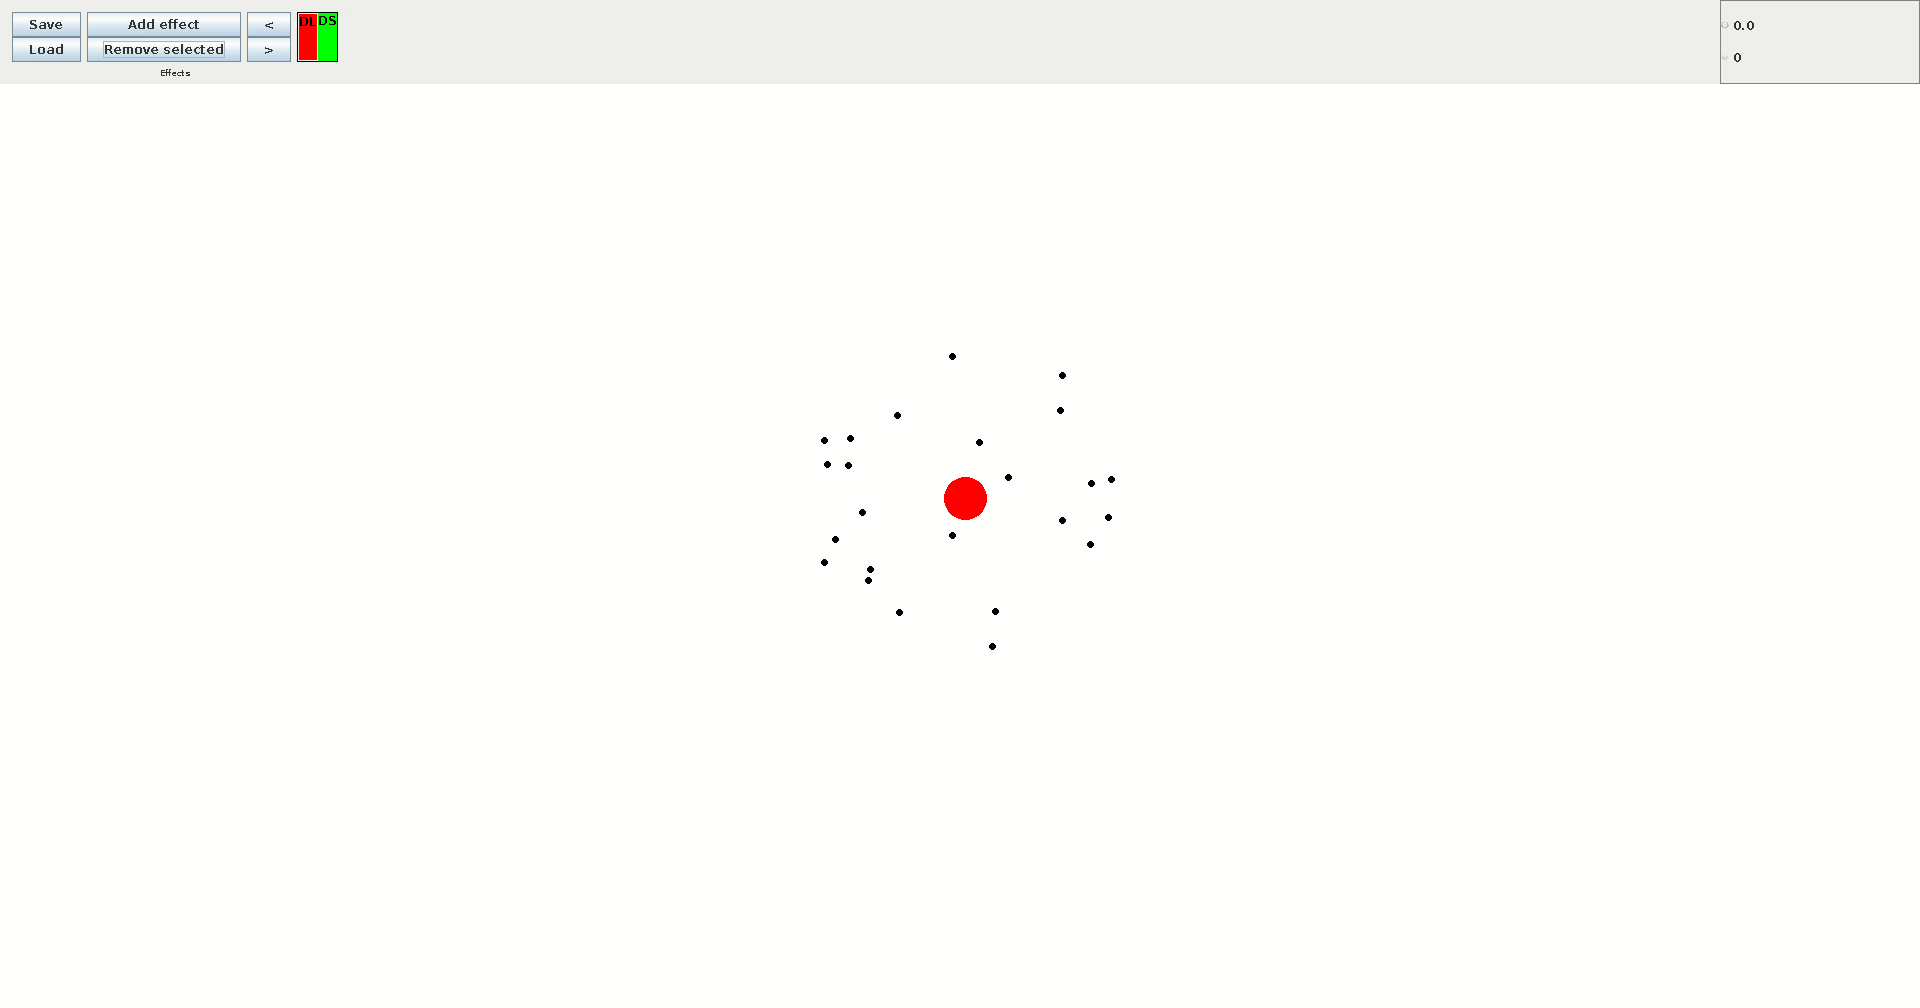
\includegraphics[width=\textwidth]{immagini/casi-studio/influence-without-groups-begin.png}
    \end{subfigure}
    \hfill
    \begin{subfigure}[b]{0.75\textwidth}
        \centering
        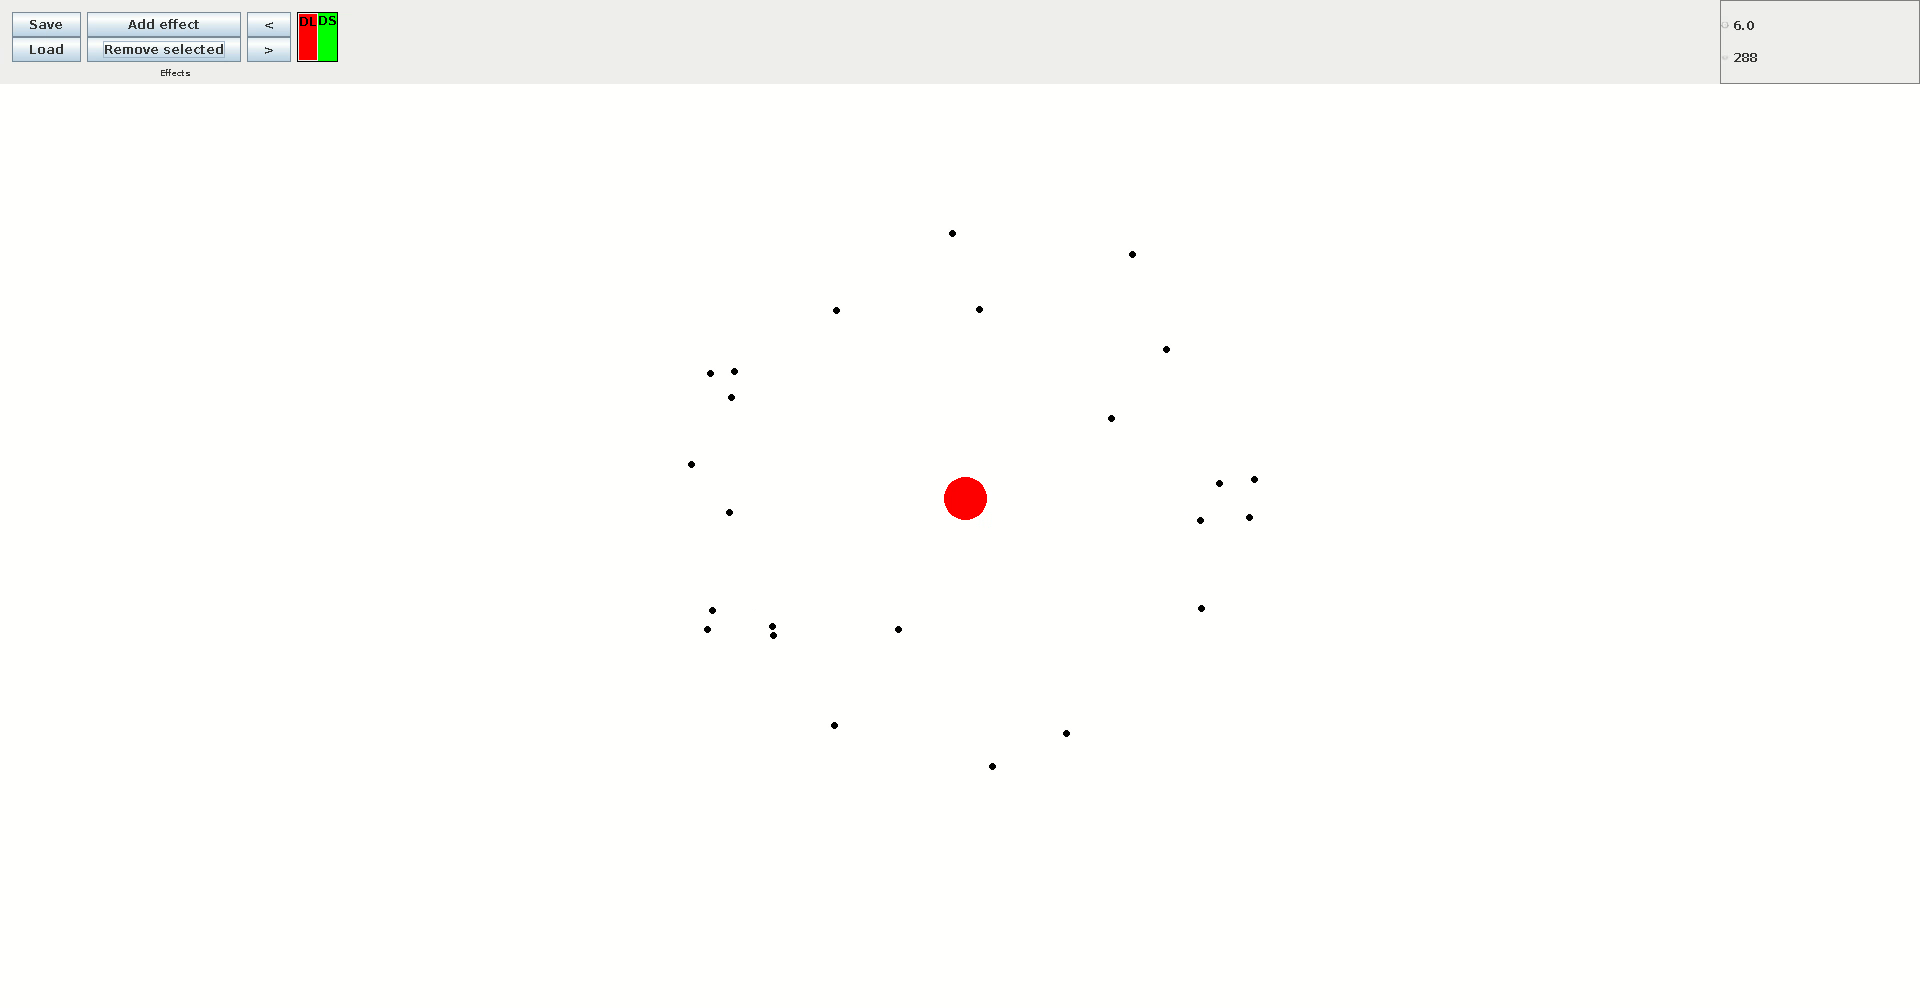
\includegraphics[width=\textwidth]{immagini/casi-studio/influence-without-groups-during.png}
    \end{subfigure}
    \hfill
    \begin{subfigure}[b]{0.75\textwidth}
        \centering
        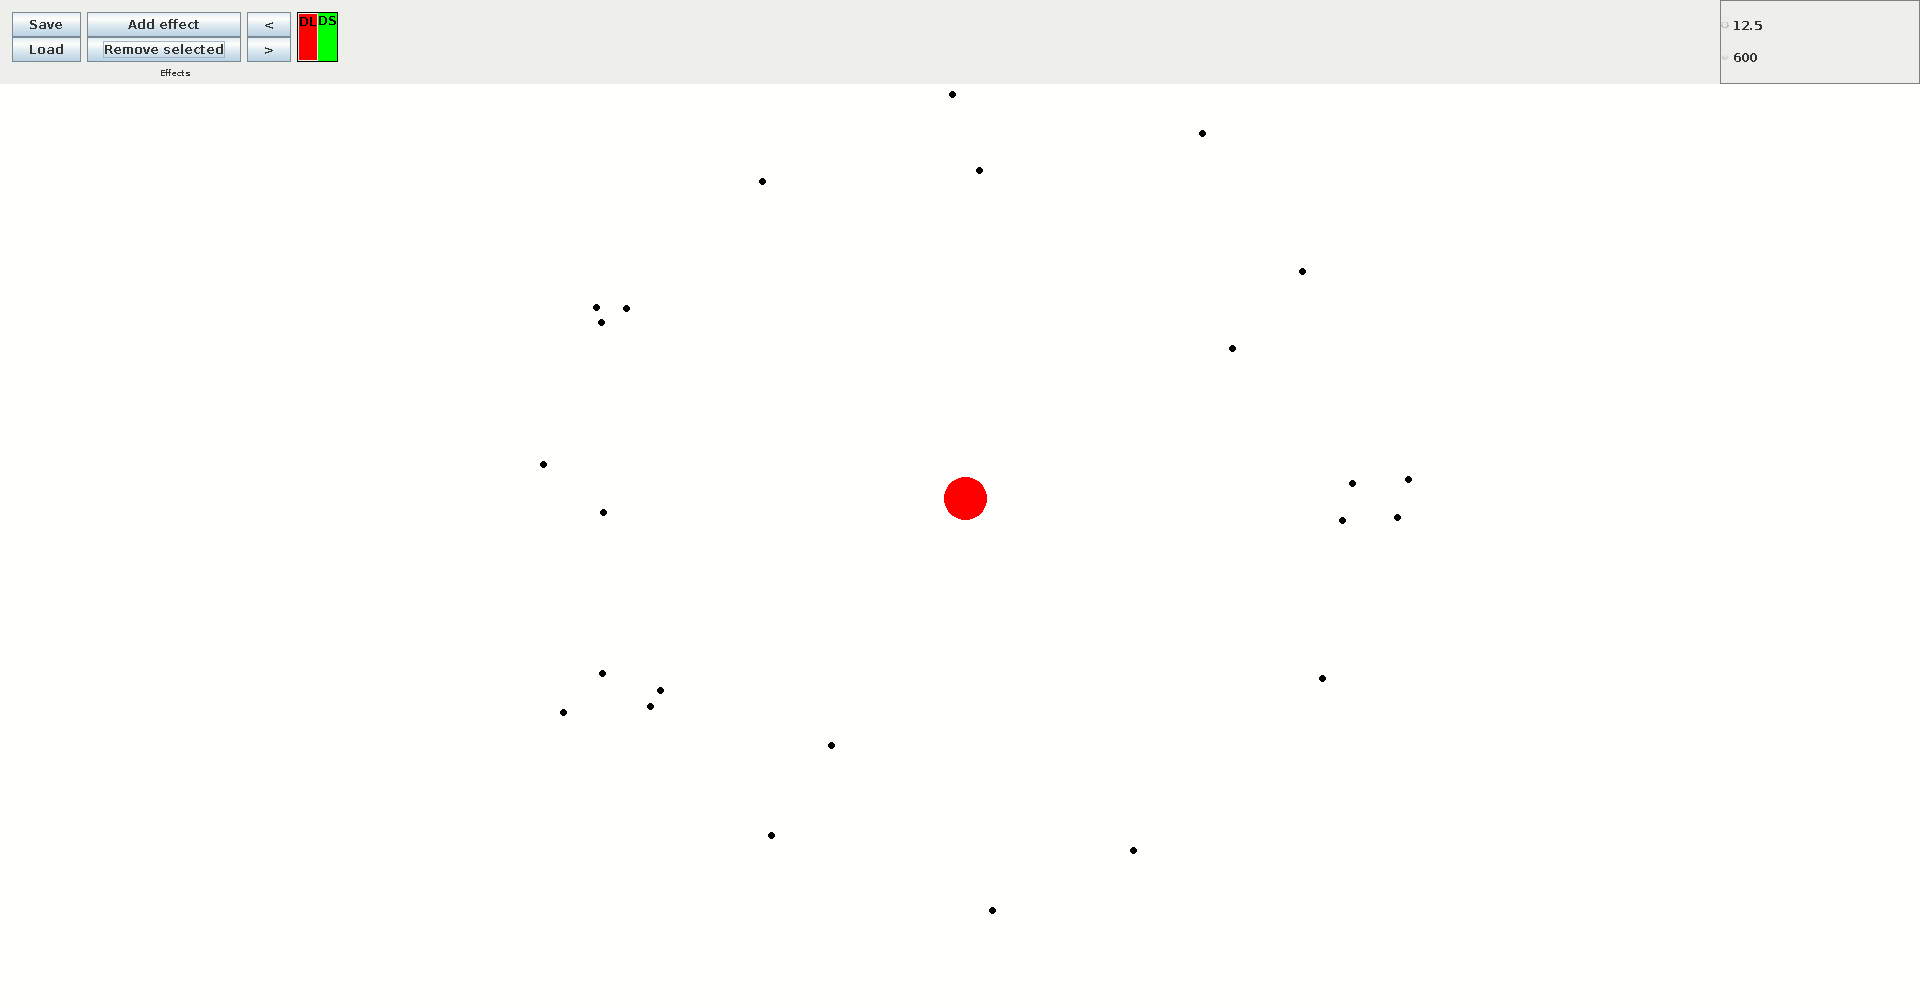
\includegraphics[width=\textwidth]{immagini/casi-studio/influence-without-groups-end.png}
    \end{subfigure}
    \caption{Fotogrammi salienti della simulazione sull'influenza del gruppo considerando pedoni solitari; è possibile notare come essi, pensando solo alla propria incolumità, si limitino a fuggire dalla zona di pericolo.}
    \label{fig:influence-without-groups}
\end{figure}

\begin{figure}
    \centering
    \begin{subfigure}[b]{0.75\textwidth}
        \centering
        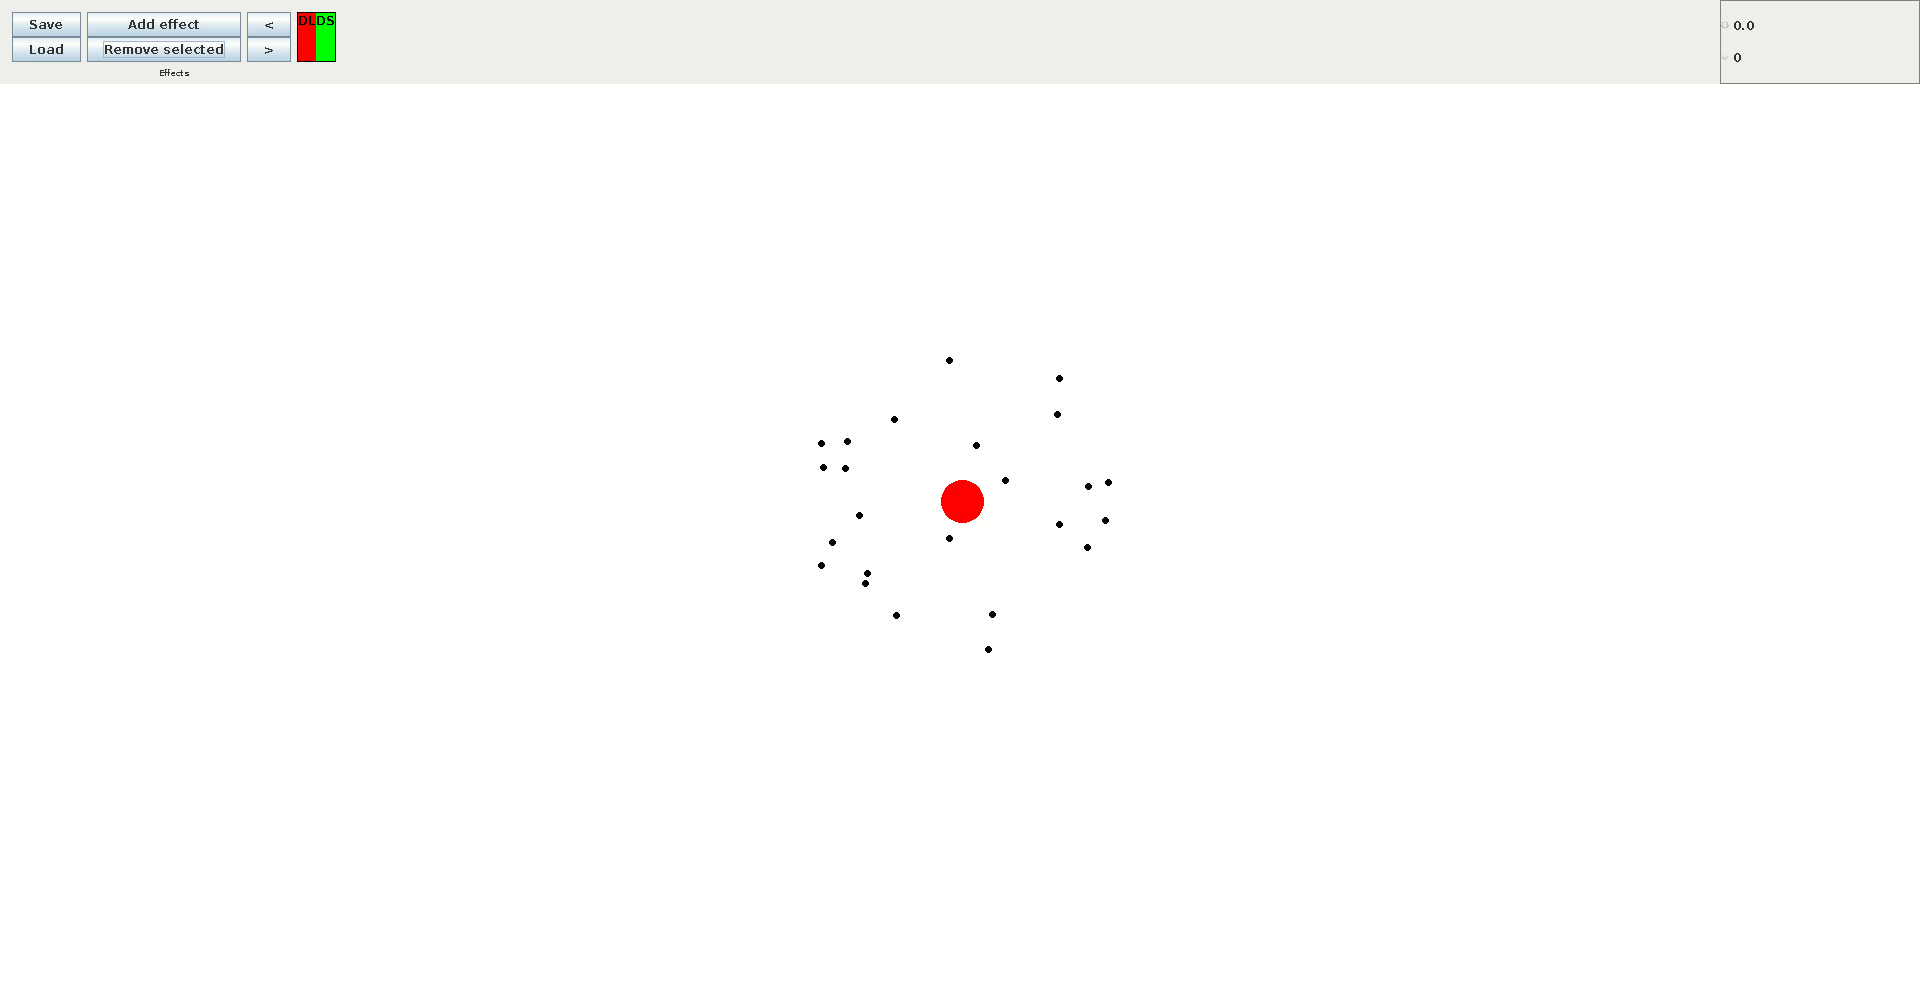
\includegraphics[width=\textwidth]{immagini/casi-studio/influence-with-groups-begin.png}
    \end{subfigure}
    \hfill
    \begin{subfigure}[b]{0.75\textwidth}
        \centering
        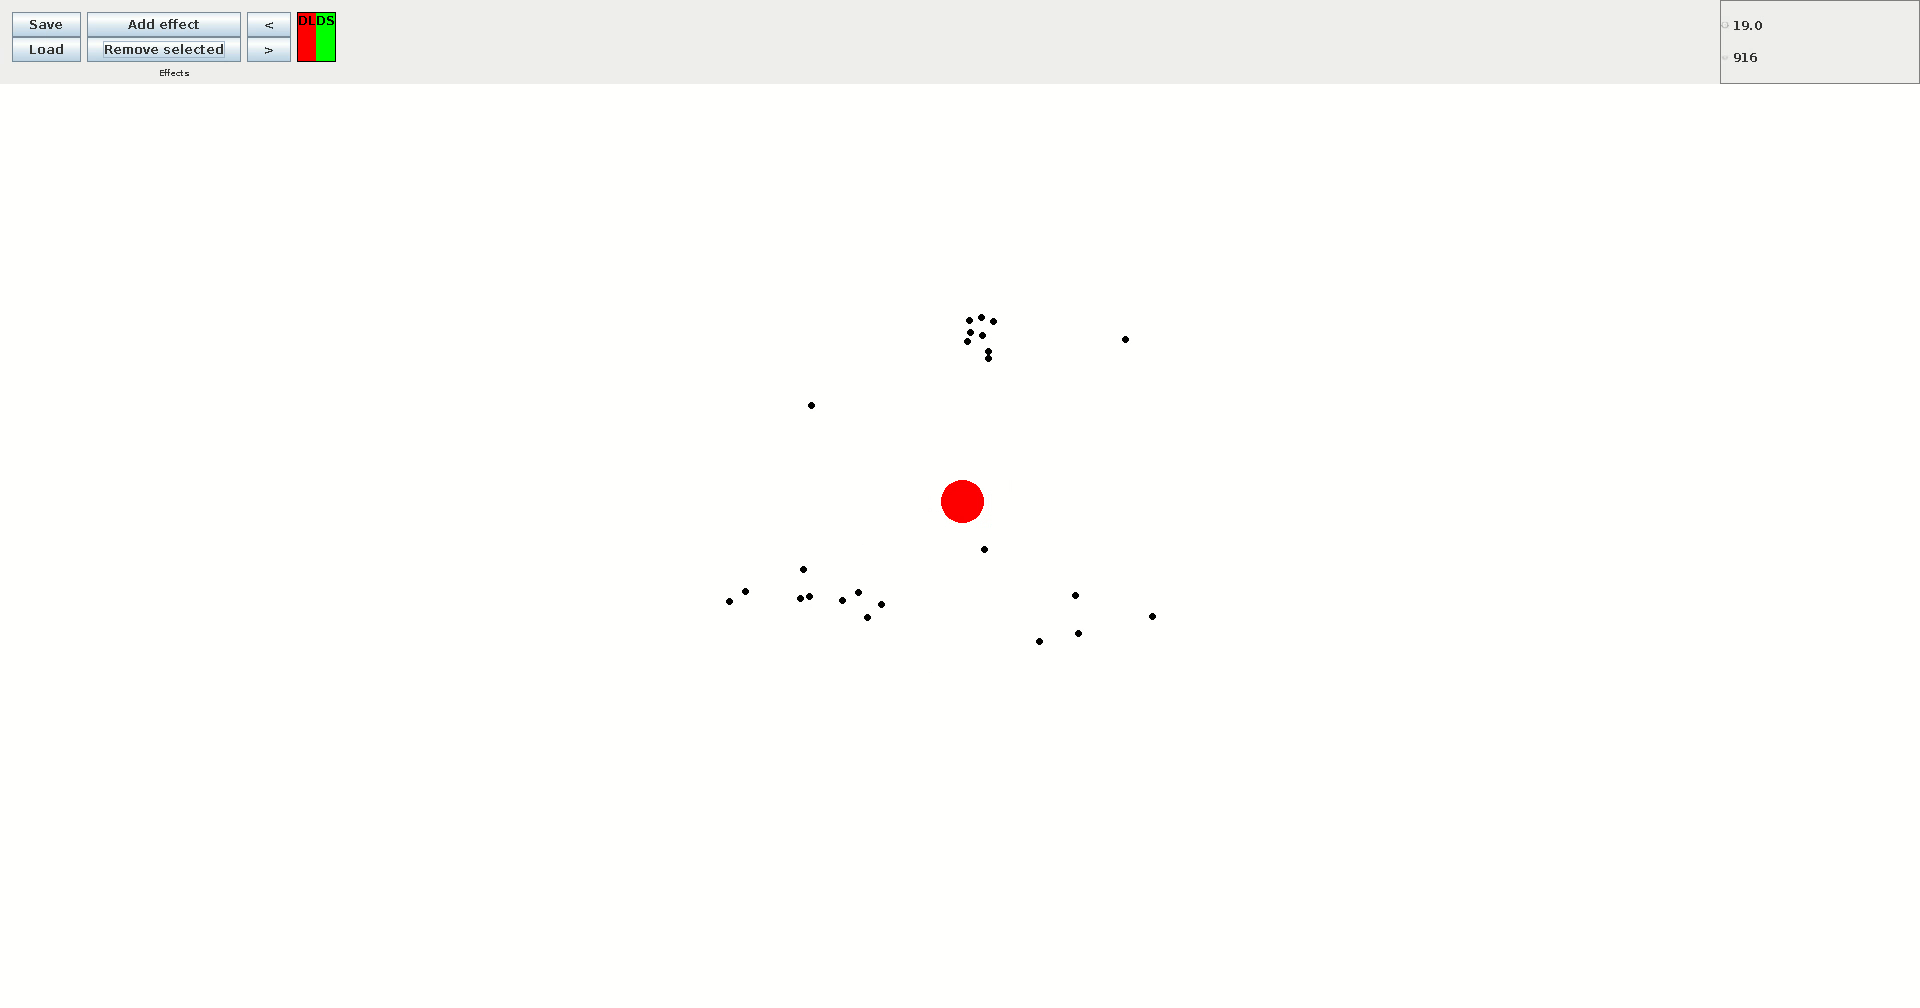
\includegraphics[width=\textwidth]{immagini/casi-studio/influence-with-groups-during.png}
    \end{subfigure}
    \hfill
    \begin{subfigure}[b]{0.75\textwidth}
        \centering
        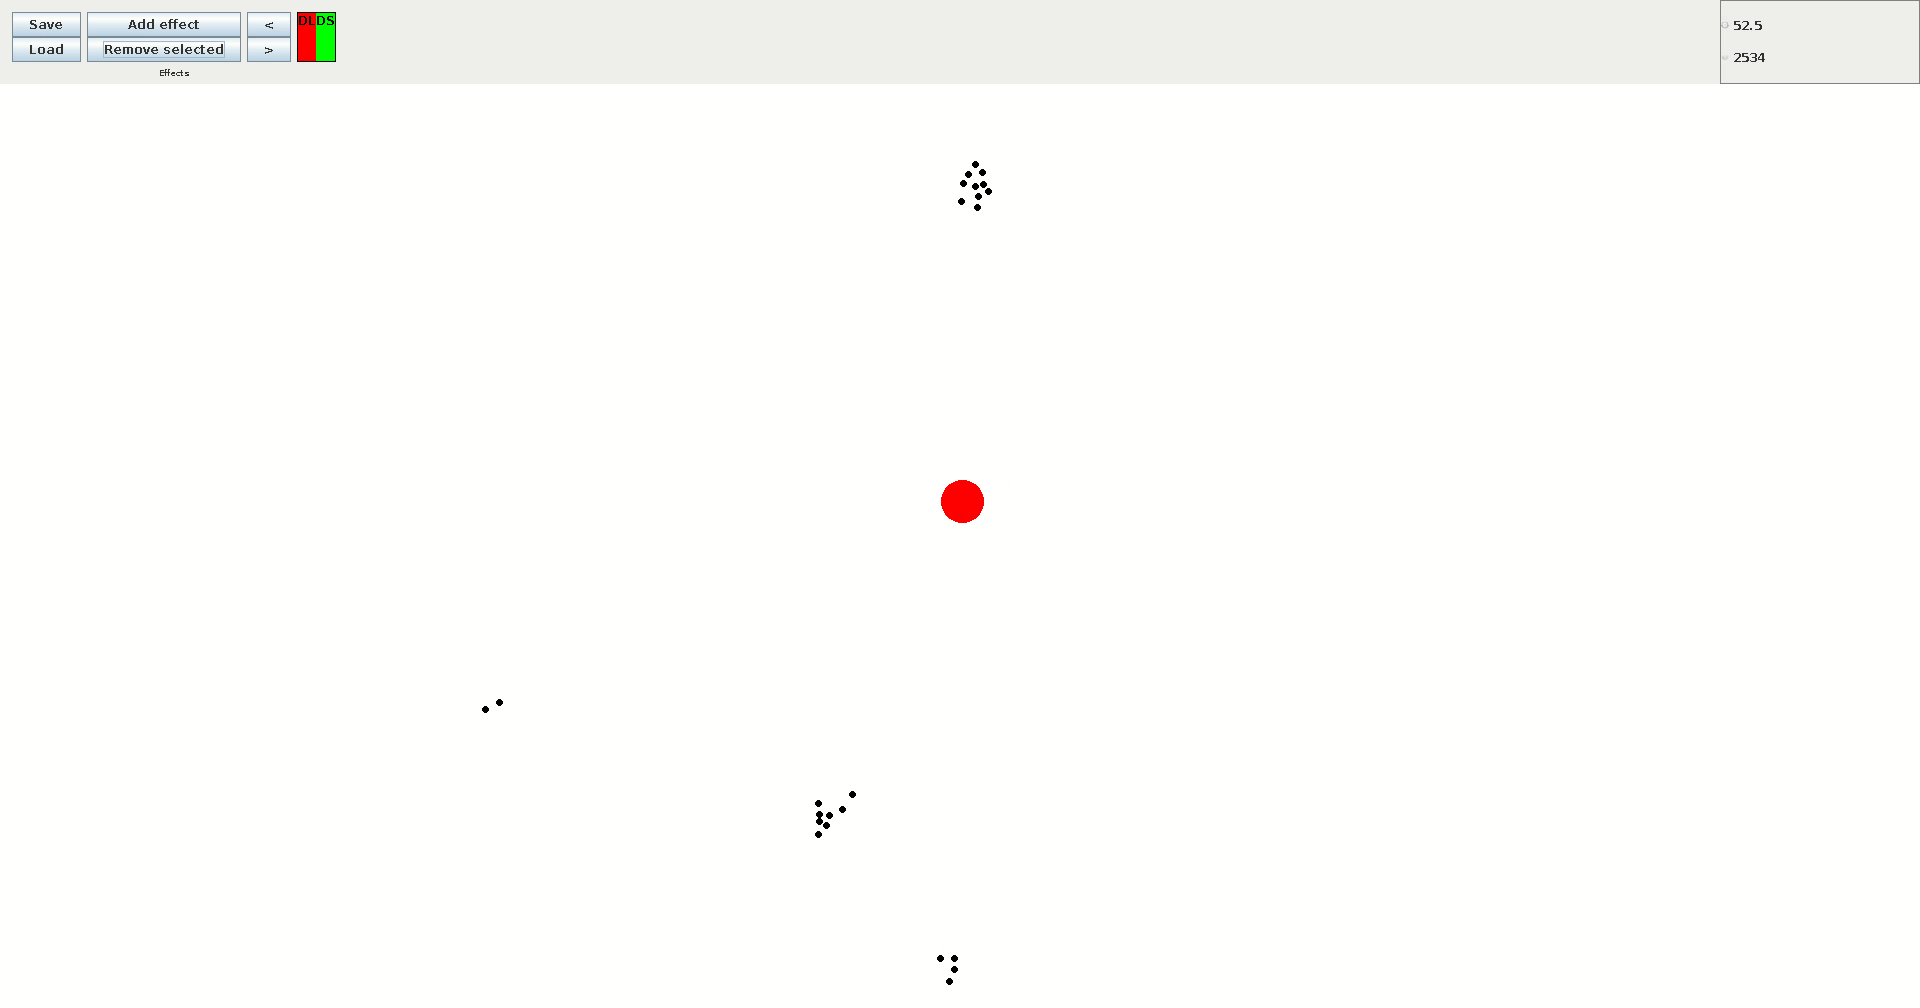
\includegraphics[width=\textwidth]{immagini/casi-studio/influence-with-groups-end.png}
    \end{subfigure}
    \caption{Fotogrammi salienti della simulazione sull'influenza del gruppo considerando quattro insiemi di amici; prima di allontanarsi dalla zona di pericolo, i pedoni cercano di riunirsi con tutti gli altri membri del loro stesso gruppo.}
    \label{fig:influence-with-groups}
\end{figure}